\chapter{Results}

\section{Step Detection}
\citet{Salvi2018} have opensourced the data used for their step detection algorithm. This includes validation data made with a ground truth device and the output of the devised algorithm on an android device. The ground truth device consisted of hardware attached to the feet of the test subjects that could exactly measure when the foot came into contact with the floor, hence when a step is taken. The use of this ground truth allows for comparison between the method devised but also with any eventual future techniques.\\
The raw data of the validation set consists of sampling time, three raw accelerometer axis signals, when a new step has been detected by the ground truth device, and step detected by the designed algorithm. The validation sets contains data of two users carrying the phones in the carrying modes outlined in \cref{sec:rw - step detection}. The device is carried in each carrying mode individually, not simultaneously. An extract of this data can be found in \cref{fig:gt_steps_vs_salvi_steps}, showing the accelerometer magnitude and points indicating the ground truth step and the steps detected by the \citet{Salvi2018} algorithm. The figure also shows how the carrying mode affects the characteristics of acceleration magnitude. For example, between carrying the smartphone in an armband and frontpocket, the former has a much more gradual change with a clear sinusoidal form, while the latter has a larger range of accelerations with much more abrupt changes. 

\begin{figure}
	\centering
	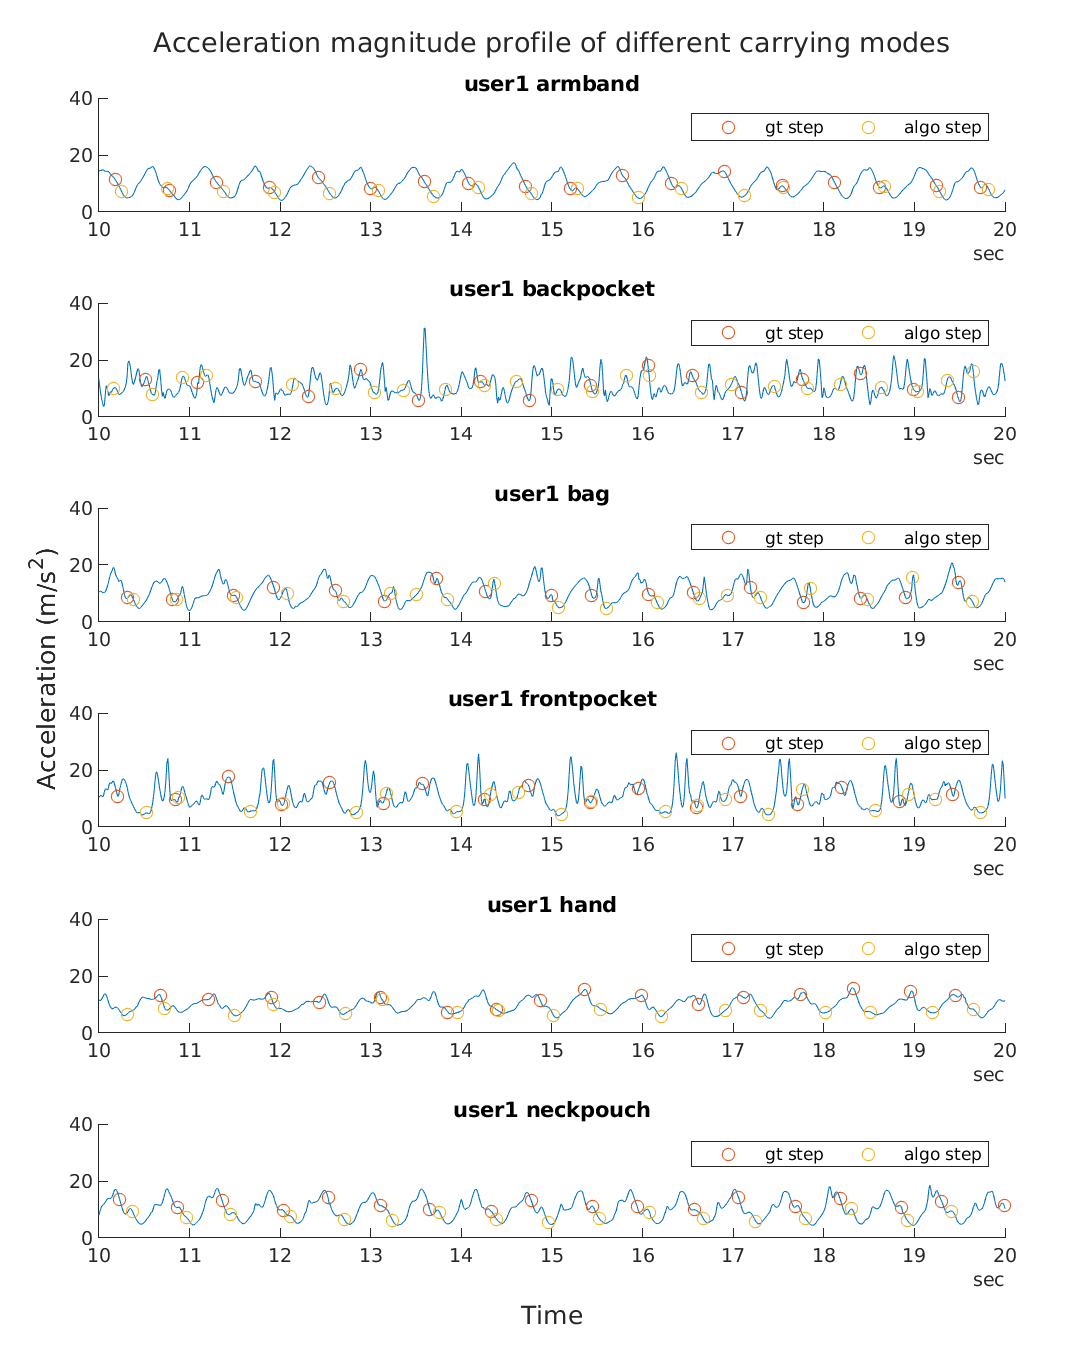
\includegraphics[width=\linewidth]{images/20200929_0951_gt_steps_vs_salvi_steps}
	\caption[Step detection validation data]{Extract of validation dataset from \citet{Salvi2018}, indicating ground truth steps and step detected by their algorithm.}
	\label{fig:gt_steps_vs_salvi_steps}
\end{figure}


The step detection method outlined in \cref{sec:meth - step detection} was applied to the validation data of the researchers, allowing for direct comparison between the ground truth and the solution of the researchers. The parameters used for the process coincide with those found by the researchers, an overview of which can be found in \cref{tab:parameters_used}.

\begin{table}
	\centering
\begin{tabular}{clc} 
	\hline
	Stage & Parameters & Value \\
	\hline & Window size & $\mathrm{M}=13$ \\
	Filtering & Filter type & Gaussian \\
	& Filter SD & 0.35 \\
	\multirow{2}{*} { Scoring } & & \\
	& Type & Mean Difference \\
	& Window size & $N=35$ \\
	Detection & Threshold & 1.2 \\
	Post-Processing & $t_{\text {window}}$ & $200 \mathrm{ms}$ \\
	\hline
\end{tabular}
\caption{Parameters used}
\label{tab:parameters_used}
\end{table}


\cref{fig:sd_comparison} shows how the method, referred to as Matlab algorithm, compares to the results in the validation datasets. \cref{fig:sd_abs_comparison} indicates the absolute number of steps detected. \cref{fig:sd_percent_comparison}  shows the percentage error compared to the ground truth, where positive percent error indicates over counting, while negative under counting. The results indicate that the method devised performs overall similarly to the method of the researchers. In some cases the error is slightly larger, as with user1 bag, while in others it is smaller as with user 2 bag. It is also apparent that with the case of user1 backpocket that there is a large percentage error for both cases. The researchers attribute this to the pocket being loose and allowing the phone to rebound when a step was taken. This would introduce nefarious components in the accelerometer signal, leading to false positives. \citet{Brajdic2013} encountered similar problems with this carrying position, hypothesizing that the relaxing of the gluteus maximus during locomotion could influence the acceleration trace.

%TODO argument why it is different than what the research achieved.

\begin{figure}[H]
	\centering
	\begin{subfigure}[t]{.5\textwidth}
		\centering
		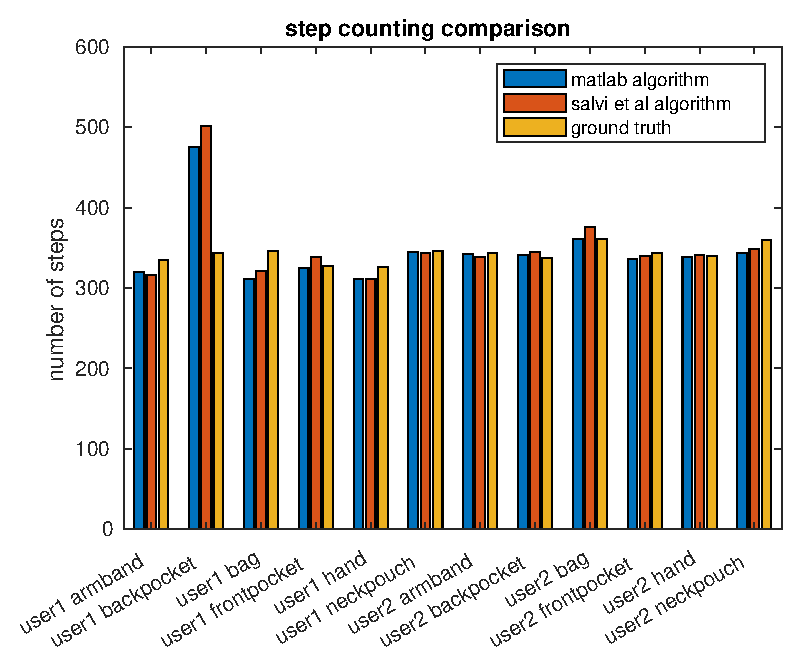
\includegraphics[width=\linewidth]{images/20200930_1214_step_counting_comparison}
		\caption{Absolute number of steps counted.}
		\label{fig:sd_abs_comparison}
	\end{subfigure}%
	\begin{subfigure}[t]{0.5\textwidth}
		\centering
		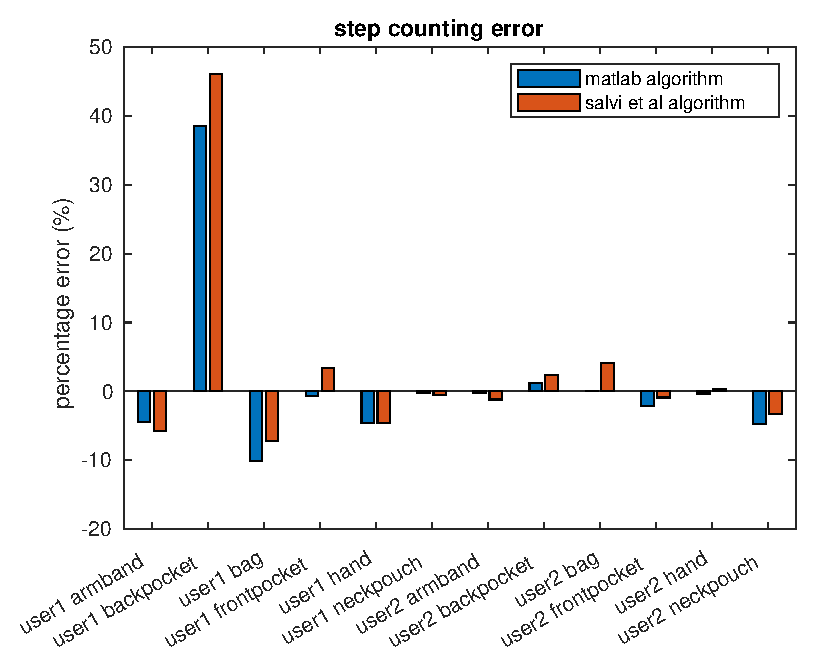
\includegraphics[width=\linewidth]{images/20200928_1248_step_counting_error}
		\caption{Percentage error from ground truth number of steps. }
		\label{fig:sd_percent_comparison}
	\end{subfigure}
	\caption[Step detection comparison]{Comparison between \citet{Salvi2018} step detection algorithm, matlab algorithm and ground truth for different carrying modes.}
	\label{fig:sd_comparison}
\end{figure}

In addition to the data made available online, original data was gathered in which a subject walked exactly 60 steps while having a smartphone in 3 different carrying modes, backpocket, frontpocket and in hand. The percentage error from the ground truth can be seen in \cref{fig:202009291013step_counting_error_of_60_steps}. Here the backpocket show similar error as with the validation data, further supporting that the method does not work reliably in this carrying position.
\begin{figure}[H]
	\centering
	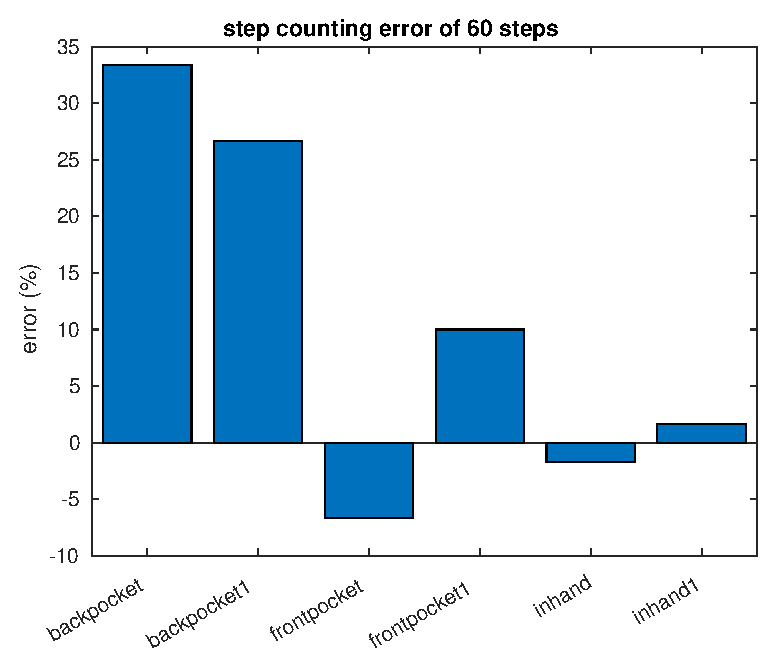
\includegraphics[width=0.55\linewidth]{images/20200929_1013_step_counting_error_of_60_steps}
	\caption{Original data step counting}
	\label{fig:202009291013step_counting_error_of_60_steps}
\end{figure}

For a PDR SHS it is not enough for the amount of steps to be accurate, but also the time when a step actually occurs. A step detection combined with the heading orientation at the moment of occurrence determines the vector in which the position estimate of the pedestrian will move. \\
In order to ascertain how both the \citet{Salvi2018} algorithm and the algorithm from \cref{sec:meth - step detection} perform in this respect, and approach to true positive step detection was determined. Since it is unrealistic to expect the step detection to be at the exact time an actual step occurs, intervals are defined where if both a step occurs and is detected, the detection counts as a true positive. If in this interval two steps are detected, both detections are not considered true positive, and are considered a true positive double count. The time interval is increase itteratively in attempt to find the highest true positive count for both algorithms. The results with the highest amount of true positives for each user and carrying mode can be found in \cref{fig:sd_tp_fp_comparison}. 

\textcolor{cyan}{discuss what the results indicate}

\begin{figure}
	\centering
	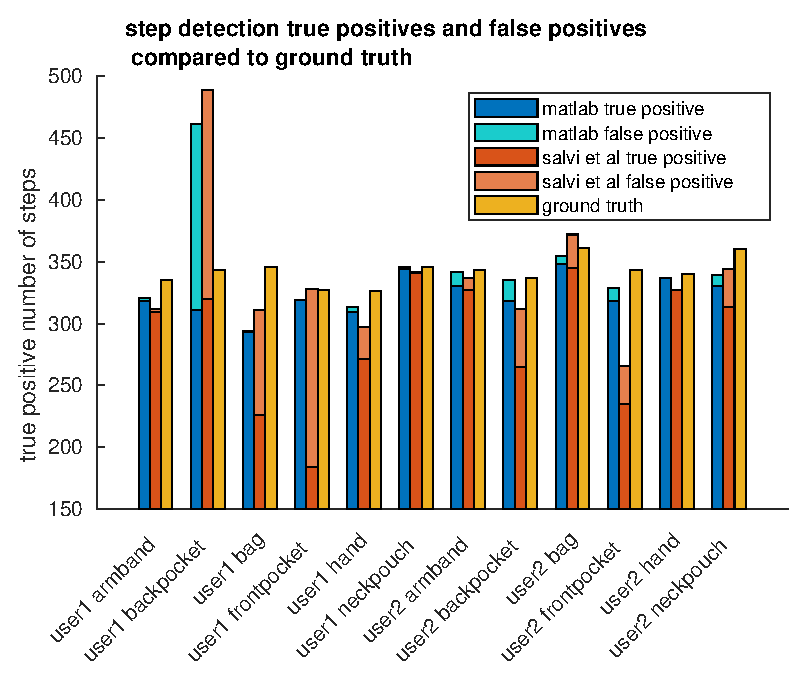
\includegraphics[width=0.7\linewidth]{images/20200930_1510_tp_fp_abs_comparison}
\caption[False positives and true positives step detection comparison]{Comparison between false positives and true positives for \citet{Salvi2018} step detection algorithm, Matlab algorithm and ground truth for different carrying modes.}
\label{fig:sd_tp_fp_comparison}
\end{figure}

\newpage

\section{Step Length Estimation}

\citet{Vezocnik2019} have also made the data they used open source. This data consist of accelerometer data of 15 different people for three walking speeds and in four smartphone carrying modes. Metrics for each test subject are collected, including height, gender and leg length. The walking modes were qualitative, in that they were either slow, normal, or fast walking speed. The carrying modes include the smartphone in pocket, in a bag, in the hand with the phone screen parallel to the floor, and in hand will swinging the carrying arm. Each person has two measurements for each combination, one for a 15 meter long straight path and another for 108 meter long straight path. The test subjects are not forced to walk these distances exactly, allowing for natural termination of their trial. \\
As done in \cite{Vezocnik2019} the smaller length set can be used to determine the parameter and the second to assess the performance.The best performing algorithm for global parameters is reiterated in \eqref{eq:Tian2016_sle2} for convenience, where $h$ is the users height and $F$ is the step frequency. 

\begin{equation}
\label{eq:Tian2016_sle2}
\text{step size} = K \cdot h \cdot \sqrt{F}.
\end{equation}

In order to determine the tunable parameter $K$ correctly for the SHS, it needs to be used with the output of the step detection algorithm. This is because step detection will have a direct effect on the step frequency. The step detection algorithm cannot guarantee that all steps are counted, potentially affecting the tunable parameter. 
From the results of step detection, the most accurate results came from holding a smartphone in the hand. This carrying mode is present in the data from \cite{Vezocnik2019}, and can therefore be used for analysis. The results are shown in \cref{fig:step_length_estimation}. Here the parameters for \eqref{eq:Tian2016_sle2} of all three walking speeds are plotted. In order to find $K$ as a universal constant a least square estimation is performed, shown by the green striped line in the plot.
\begin{figure}[H]
	\centering
	\begin{subfigure}[t]{.45\textwidth}
	\centering
	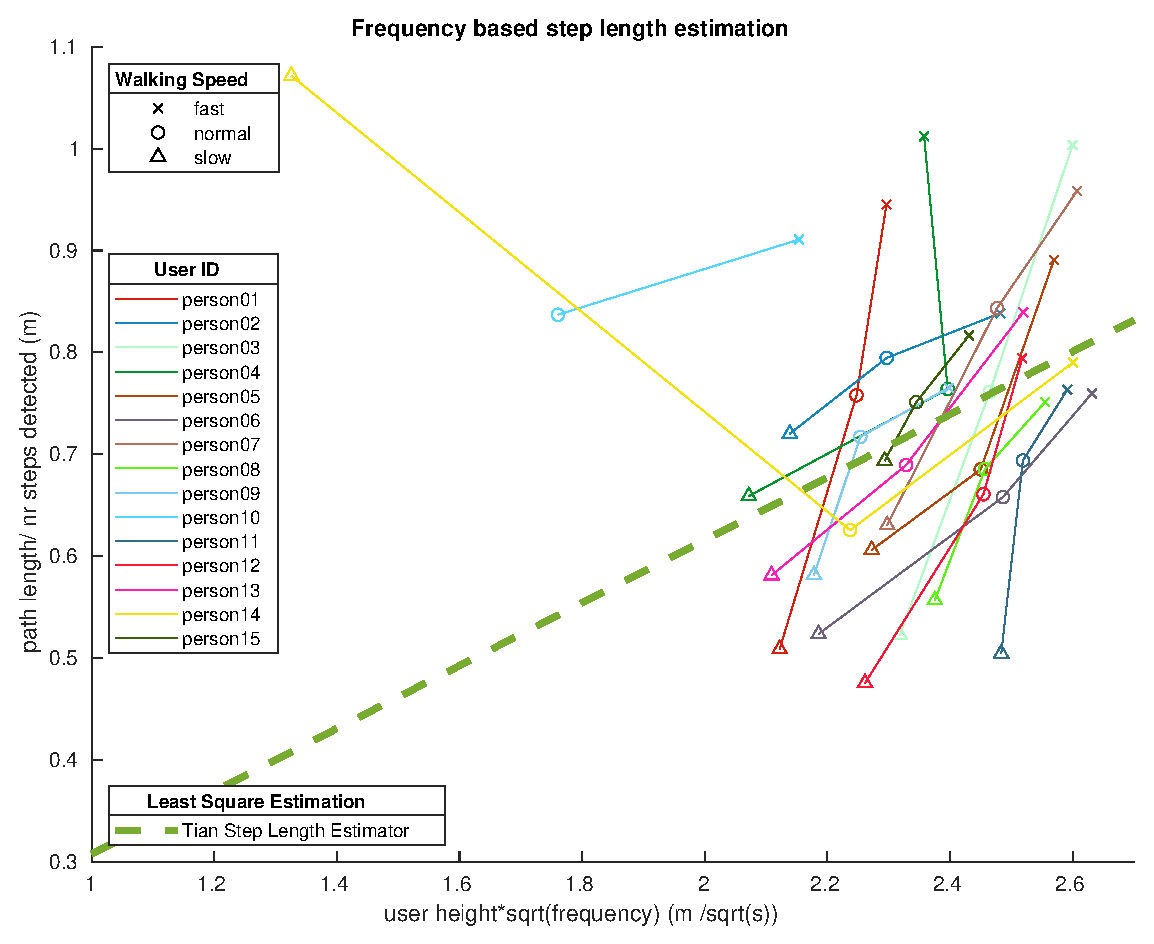
\includegraphics[width=\linewidth]{images/20201028_1050_step_length_all_data}
	\caption{step length estimation constant = 0.3116}
	\label{fig:step_length_all_data}
	\end{subfigure}
	\begin{subfigure}[t]{.45\textwidth}
		\centering
		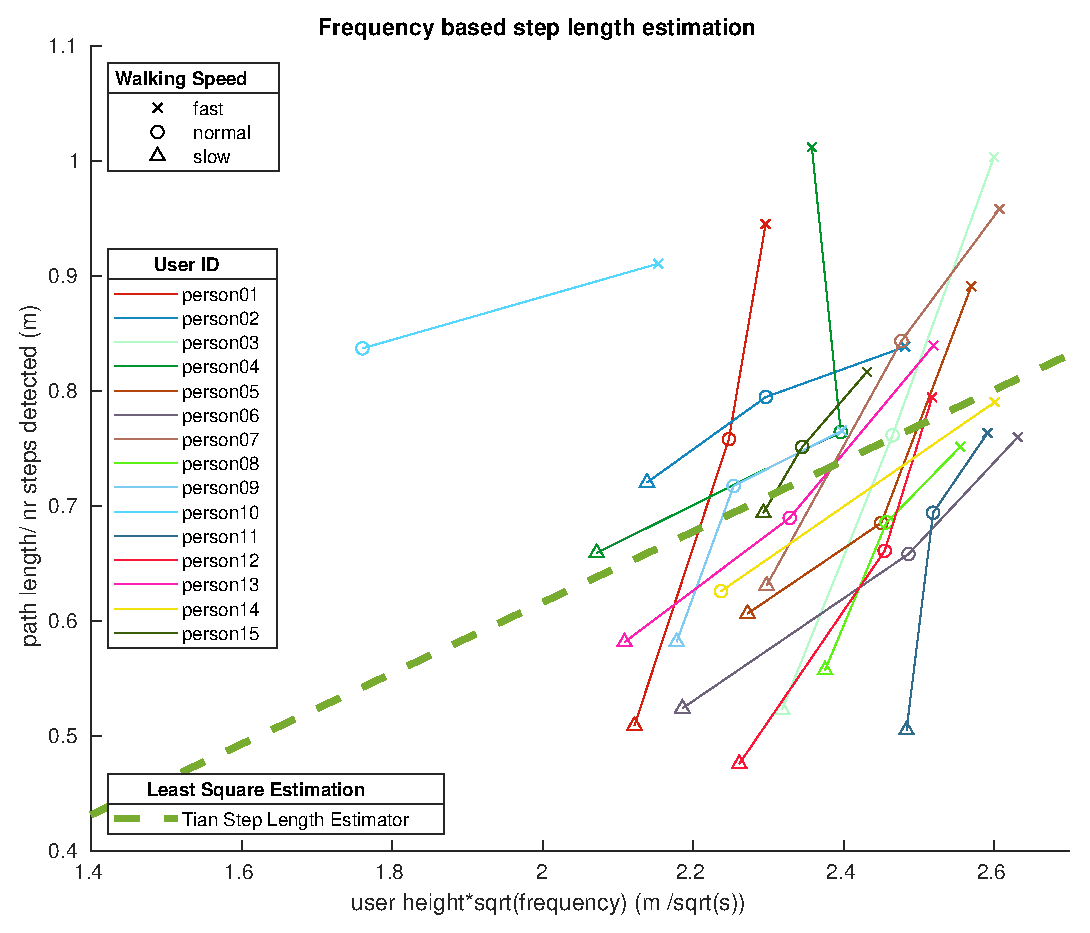
\includegraphics[width=0.95\linewidth]{images/20201028_1051_step_length_good_data}
		\caption{step length estimation constant = 0.3080}
		\label{fig:step_length_without_faults}
	\end{subfigure}
	\caption{step length estimation}
	\label{fig:step_length_estimation}
\end{figure}
Using the open source data has not come without problems, as can be seen in \cref{fig:step_length_all_data}. While most data seems to have relatively good step detection, there are two samples that do not conform to the general trend suggesting that step detection is not working correctly. The two potentially faulty data points are the slow walking sample of both person 10 and 14. For the former, no steps have been detected and is therefore not visible in the plots, while for the latter too little steps have been detected. For person 14, 14 steps have been detected for slow walking, which is less steps than when the subject was walking fast. This clearly suggests that a wrong step detection occurred. It is difficult to determine why this is occurring since the exact details. It could be that during this sample, the test subject was holding the phone incorrectly, the person had a very different step strategy when performing at this speed, or the phone was malfunctioning. This outlier affects the eventual tunable parameter. Removing it will change the estimate, as shown in \cref{fig:step_length_without_faults}. The performance of the step length estimate can be checked by using the validation dataset, where all users walked a longer distance, but with the same experimental setup. Here the accelerometer data can be passed through step detection and step length estimation to estimate the total distance traveled. This can then be compared with the actual distance traveled to determine the error. The data can also be used to determine if the difference in tunable parameter has a significant affect on the estimate. The results are found in  \cref{fig:step_length_estimation_validation}, where the absolute distance error for all walking speeds for all test subjects are shown, indicated by the dataset ID.
\begin{figure}[H]
	\centering
	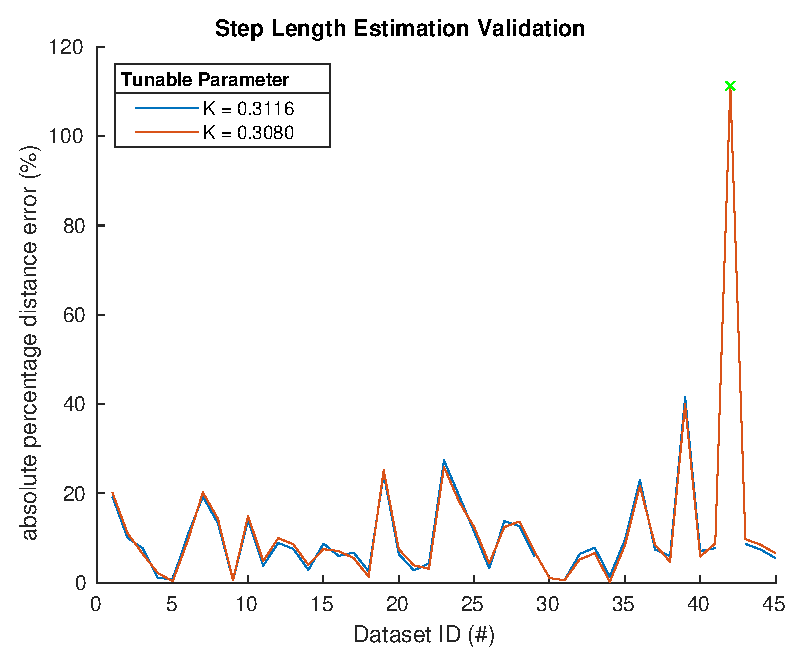
\includegraphics[width=0.6\linewidth]{images/20201028_1344_Step_Length_Estimation_Validation}
	\caption{Step length estimation using validation dataset}
	\label{fig:step_length_estimation_validation}
\end{figure}

What is noticeable from the results is that there is a large outlier. This is with dataset 42, which corresponds to the slow walking speed of test subject 14, which is also the setting in which the tunable parameter estimation had an outlier. This further supports that there is something significantly different when this test subject is performing at this walking speed. With this outlier the mean absolute error is 11.8 percent with a standard deviation of 17.1 percent. Without the outlier, the mean absolute error is 9.7 percent with a standard deviation of 8.0 percent. Both results are worse than those cited by \cite{Vezocnik2019}, which indicate a mean of 7 percent with a standard deviation of 5 percent.
The results also indicate that the different tunable parameters do not make a significant difference in accuracy. The difference in performance is likely to the difference in step detection, which the research do specify exactly. \par 
A similar smaller scale experiment was performed with three different people also walking at three different walking speeds. The results can be found in \cref{fig:step_length_personal_testing}. 
\begin{figure}[H]
	\centering
	\includegraphics[width=0.5\textwidth]{example-image-a}
	\caption{Original data step length estimation}
	\label{fig:step_length_personal_testing}
\end{figure}

{\color{cyan} still need to add comment on results of test with original data and see how it compares with the data from \cite{Vezocnik2019}... The results so far show that general parameters are not good. In the experiments indoor }

\textcolor{red}{I think that step length estimation is one of the largest error sources ATM. Is it work while switching to a different technique? \citet{Vezocnik2019} also indicate on that is good for personalized parameters ....? I think that this could be fixed quickly}

\section{Indoor Experiments}

Due to restriction caused by the COVID-19 pandemic, indoor testing was located at the house of a family member. The test consisted of walking around indoors with a smartphone in hand, and recording the IMU signals in the phone through an app, while also filming the path that is being walked. During the experiment a smartwatch was worn around of the not smartphone hand and used to open doors. This opening of doors was also recorded using the app running on the smartphone, which had a button to record timestamps. The full experimental process can be found in \cref{appendix:shs_experiment}. \par 
In order to use map information with the particle filter, different sources were combined to generate a map. Rudimentary paper blueprints of the building were available and could be photographed and traced in software to generate a picture of the indoor environment. This image has clear color distinction between the different structures within the building, including walls, doors and furniture. The positioning and size of furniture was estimated. The final image is seen in \cref{fig:indoor_blueprint}. This image is in pixel coordinates and needs to be transformed into meter coordinates. It then needs to represent a 2D probability density function so that it can be used in the particle filter measurement update. \\
The OccupancyMap in the MATLAB Robotics Tool box is suitable for this. An occupancy grid is a grid in which each cell has a value representing the probability of the occupancy of that cell. By measuring a known structure in Google Maps using the measurement tool and comparing with its pixel length in the image, a meter to pixel ratio can be defined. The Google Maps measurement can be found in \cref{fig:house_google_maps}. This pixel to meter ratio combined with the image, allows MATLAB to generate an occupancy grid as shown in \cref{fig:pf_map}. This same process can be used to get the meter position of all doors.

\begin{figure}[H]
	\centering
	\begin{subfigure}[t]{.3\textwidth}
	\centering
	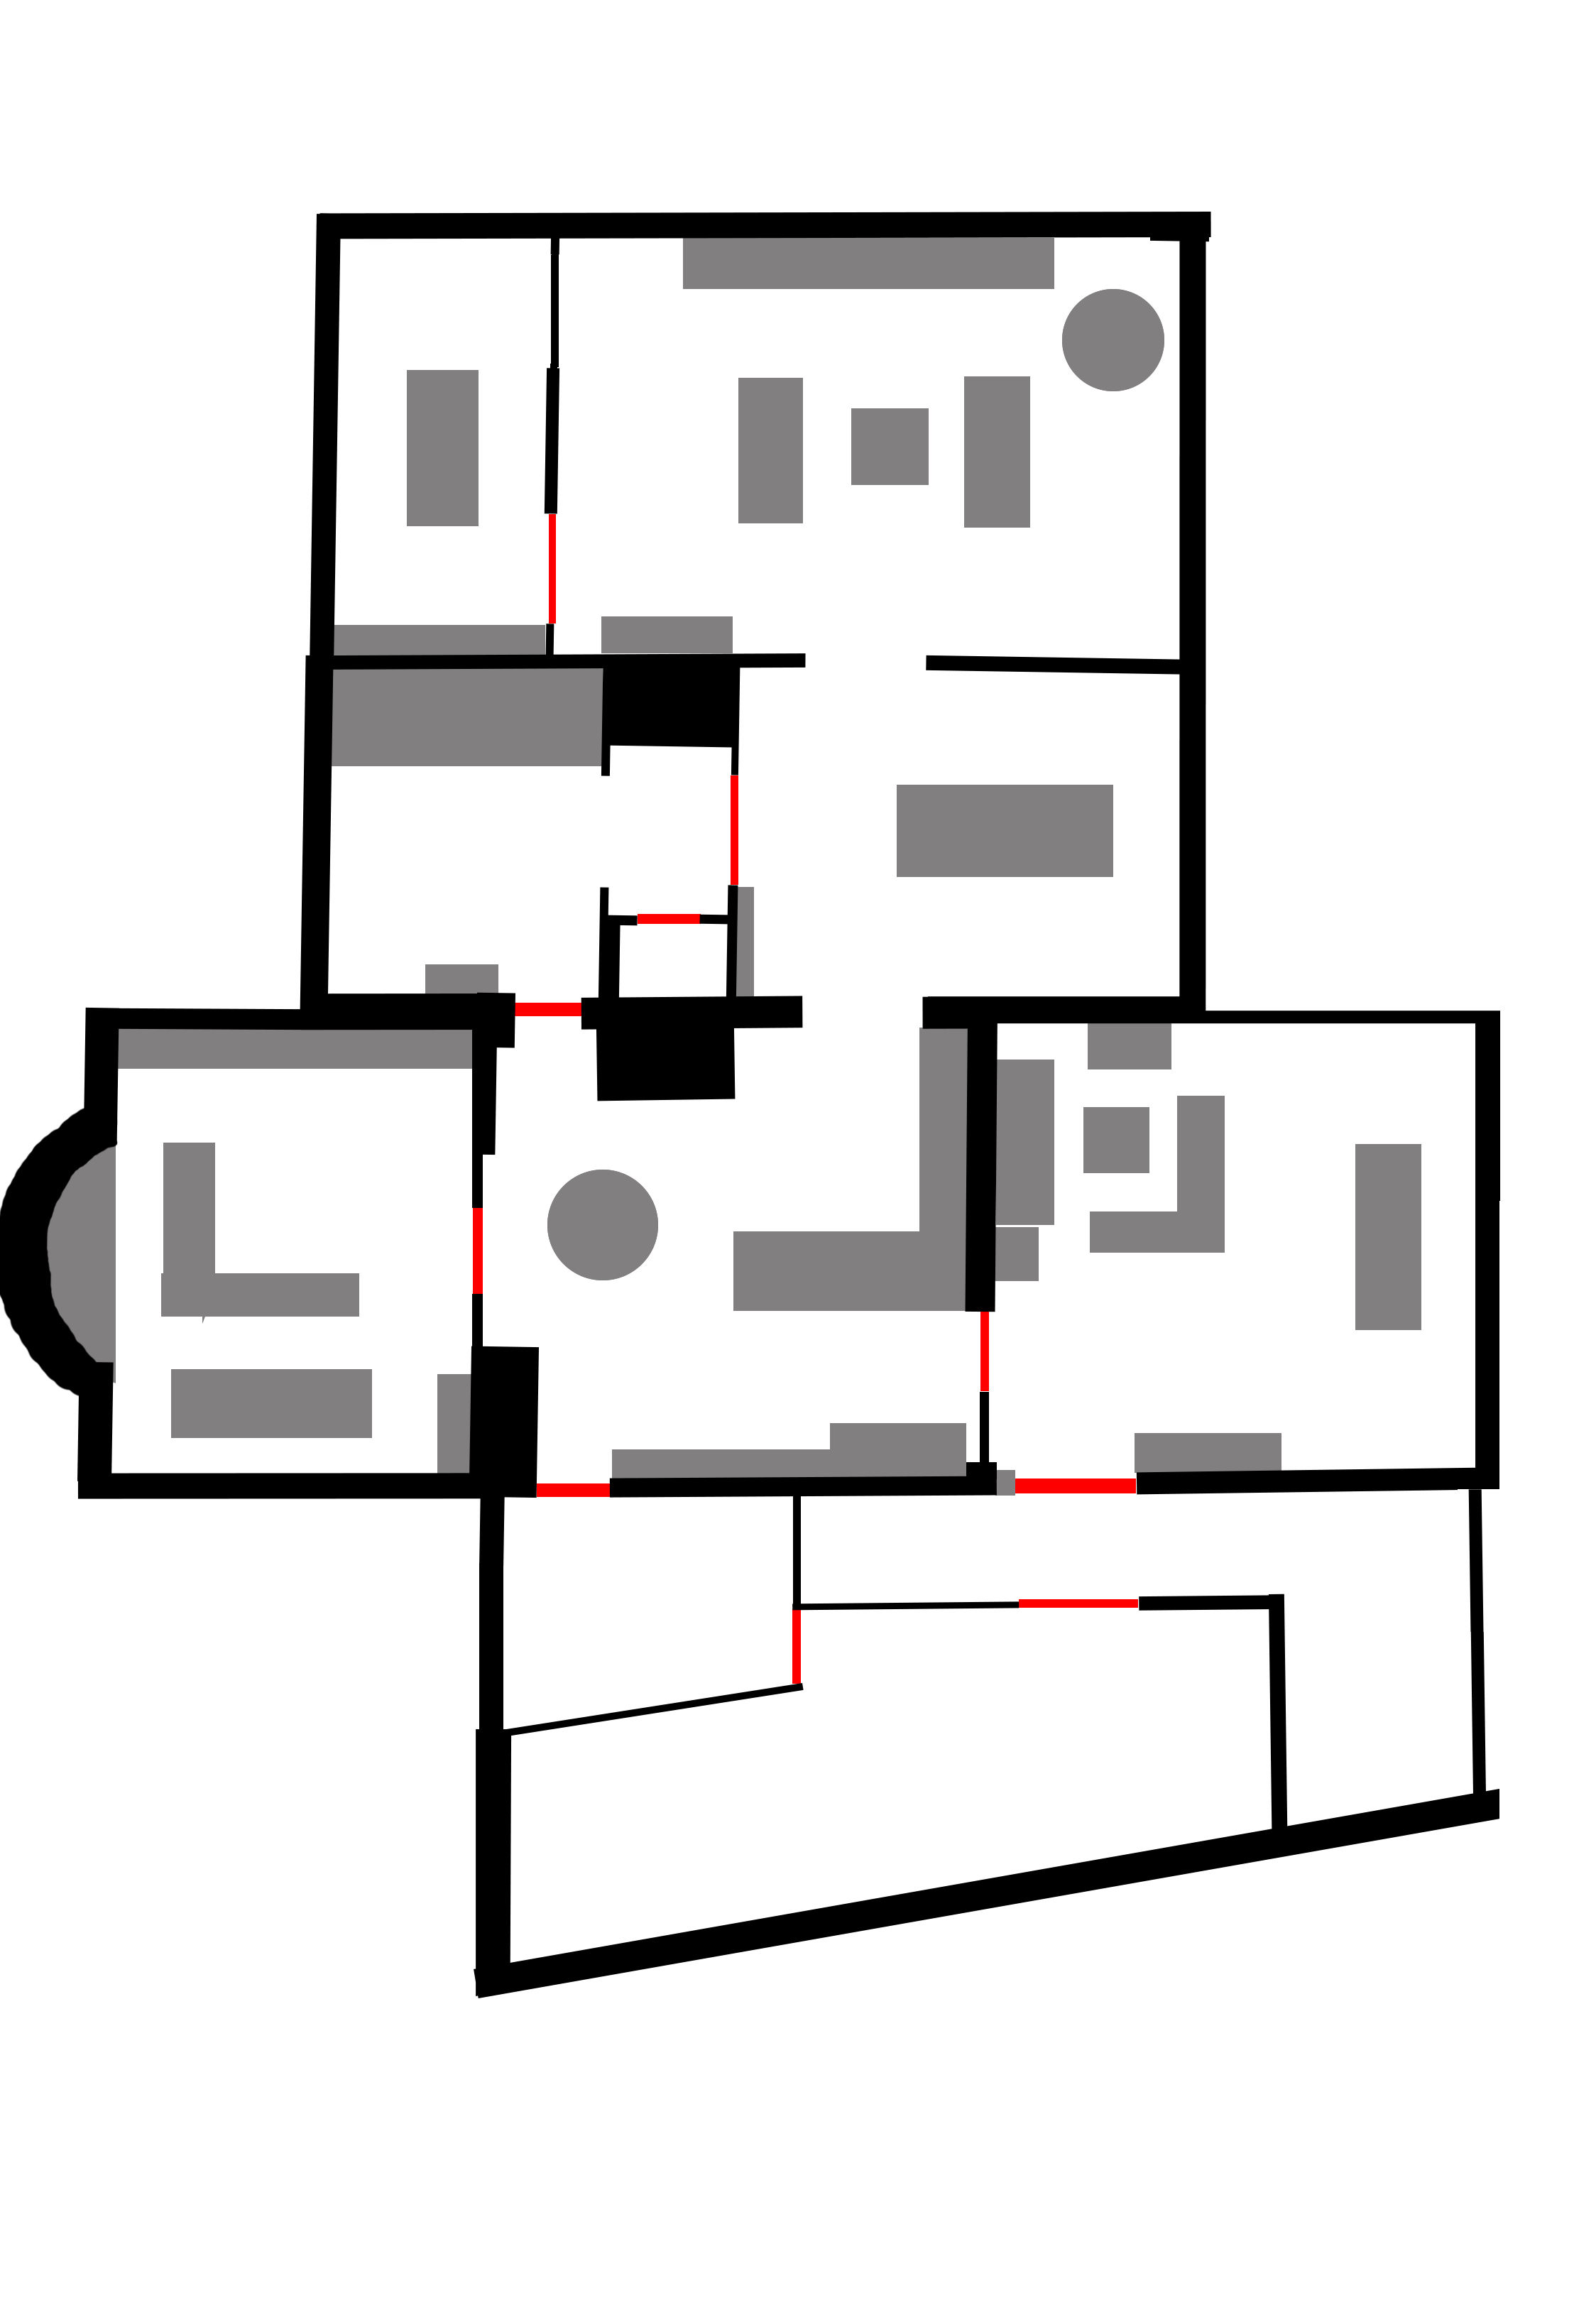
\includegraphics[width=0.9\linewidth]{images/indoor_blueprint}
	\caption[Image from building blueprints]{Image from building blueprints. Black, grey and red represent walls, furniture, and doors, respectively.}
	\label{fig:indoor_blueprint}
\end{subfigure} \quad
\begin{subfigure}[t]{.3\textwidth}
	\centering
	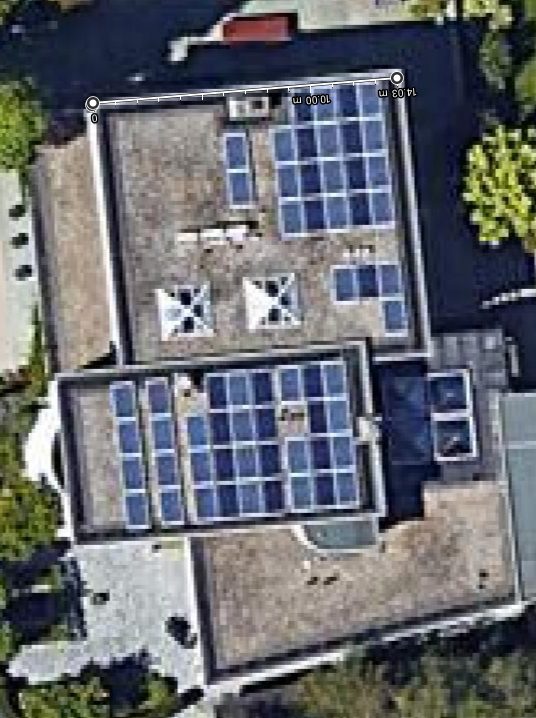
\includegraphics[width=0.9\linewidth]{images/house_google_maps}
	\caption{Measurement from Google Maps}
	\label{fig:house_google_maps}
\end{subfigure} \quad
\begin{subfigure}[t]{.3\textwidth}
	\centering
	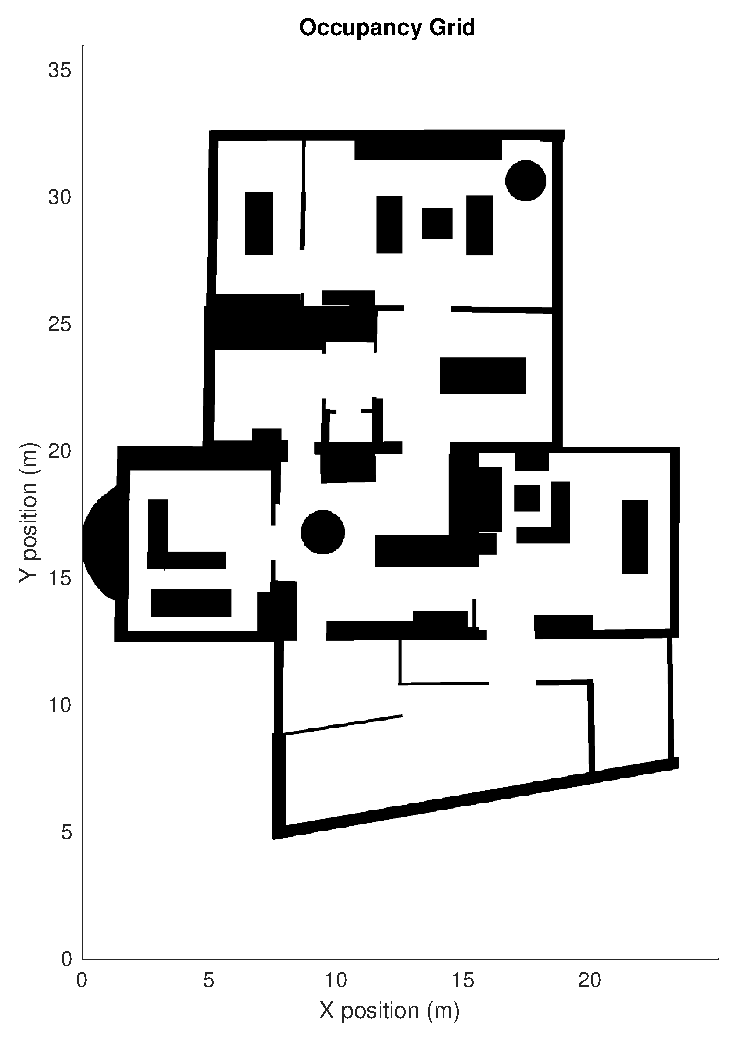
\includegraphics[width=0.9\linewidth]{images/20201030_1157_pf_map_1}
	\caption{Particle Filter map result}
	\label{fig:pf_map}
\end{subfigure}
\label{fig:particle_map_construction}
\caption{Particle filter map creation}
\end{figure}

During the experiment, a total of 8 trials were walked by one test subject, each trying to generate a different trajectory than the previous trials. The video recorded during the experiment can be used in postprocessing to get a ground truth. This was done by replaying the video and at set intervals manually indicating approximately where on the map the test subject was located. The position and time elapsed were recorded. The output of these trials can be used to test certain SHS components individually and the system as a whole.



\subsection{Indoor Orientation Estimation}
The indoor orientation estimation method outlined in \cref{sec:method-EKF} can be compared with the output of the android operating system. Two examples can be found in 

\begin{figure}[H]
	\centering
	\begin{subfigure}[t]{.45\textwidth}
	\centering
	\includegraphics[width=0.7\textwidth]{example-image-a}
	\caption{Orientation estimation of trial 1 compared to android orientation estimation}
	\label{fig:trail1 - shs}
\end{subfigure}\quad
\begin{subfigure}[t]{.45\textwidth}
	\centering
	\includegraphics[width=0.7\textwidth]{example-image-b}
	\caption{Orientation estimation of trial 2 compared to android orientation estimation}
	\label{fig:trail2 - shs}
\end{subfigure}
\end{figure}

These two examples indicate that the two estimation techniques have a similar performance. There is no reason for a direct comparison between the orientation estimation outline in \cref{sec:method-EKF} and the attitude estimation of the, since this will be relative to each other and not to the ground truth which is not available. 

A rudimentary comparison could be made using the ground truth of the experiment, where the assumption is made that the angle of the displacement vector can be considered the orientation of the phone. The different orientations can be compared by showing the difference in angle for the initial orientation. An example of this can be found in \cref{fig:orientation_comparison}, also showing the orientation estimations of the phone and the EKF method.

\begin{figure}[H]
	\centering
	\includegraphics[width=0.6\textwidth]{example-image-c}
	\caption{Orientation distilled from ground truth compared to orientation estimation of android system and EKF}
	\label{fig:orientation_comparison}
\end{figure}

The error between each trial and the orientation distilled from the ground truth trajectory can be found in \cref{fig:orientation_error_comparison}.

\begin{figure}[H]
	\centering
	\includegraphics[width=0.6\textwidth]{example-image-c}
	\caption{Error between ground truth orientation and android system and EKF}
	\label{fig:orientation_error_comparison}
\end{figure}


{\color{red}As can be seen this plot has not been generated yet. Depending on the outcome a comparison can be made over all trials to determine performance of the different methods. What do you think, is this a valid way of comparing orientation estimate?}


\subsection{Step Length Estimation}

\textcolor{red}{is it worthwhile to compare step length estimation with the video ground truth generated?}

\subsection{Step and Heading System}

\textcolor{cyan}{trial naming at this point is not consistent, also not in the plots ... needs to be changed}

All components of the step and heading system have been tested separately, giving an indication of their strengths and limitations. Now the whole system can be combined and tested in an indoor environment to evaluate the complete system performance.
For every trial the smartphone IMU data is passed through the different components of the SHS outlined in this report. Each trajectory can then be compared to the ground truth generate through post processing as outlined at the beginning of this section. Two trials with their trajectory projected onto the map and side by side comparison with the ground truth can be found in \cref{fig:trial1_shs_gt_comparison} and \cref{fig:trial2_shs_gt_comparison}. Note that the shs trajectories in these images have been rotated heuristically in order to fit the map as best as possible. This needs to be done since there is no way for the step and heading system output to know how to orient itself with respect to the building. This is because it does not have pre-existing knowledge on the orientation of the magnetic field inside the building. Since this heuristic rotating is only used to give an indication of the shs output compared to the ground truth, it is not possible to compare it quantitatively with the ground truth, since it is not a standalone solution for indoor localization.

\begin{figure}[H]
	\centering
	\begin{subfigure}[t]{.45\textwidth}
		\centering
		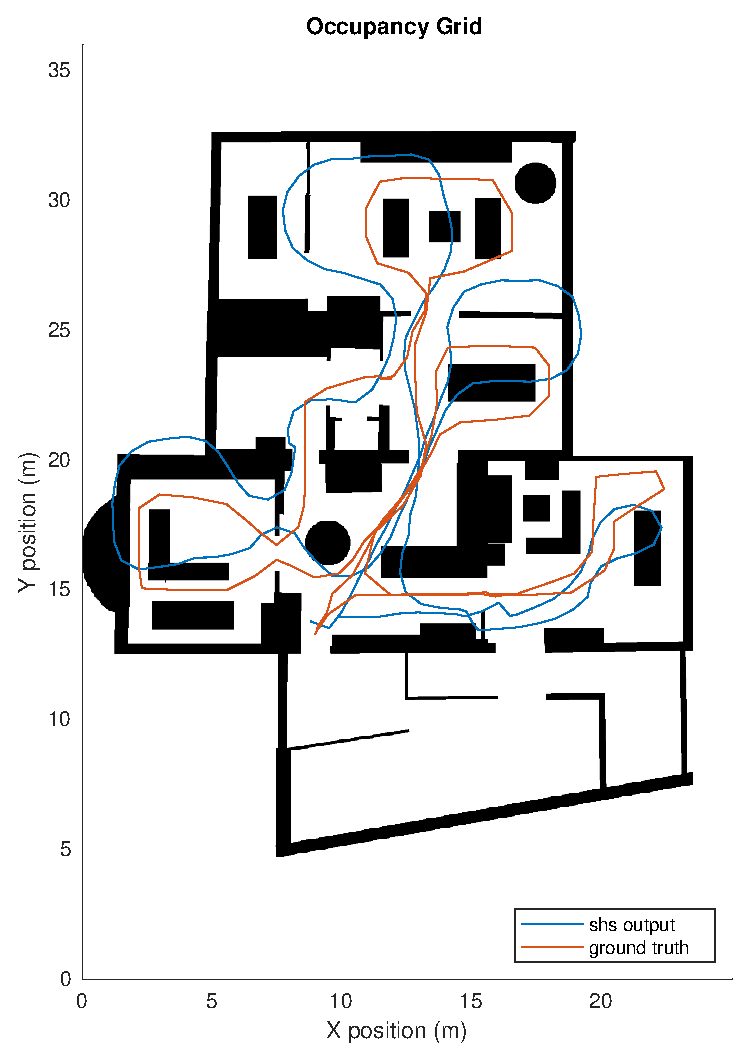
\includegraphics[width=0.9\linewidth]{images/20201029_1040_trial1_shs_1}
		\caption{trajectory comparison}
		\label{fig:trial1_on_map}
	\end{subfigure}
	\begin{subfigure}[t]{.45\textwidth}
		\centering
		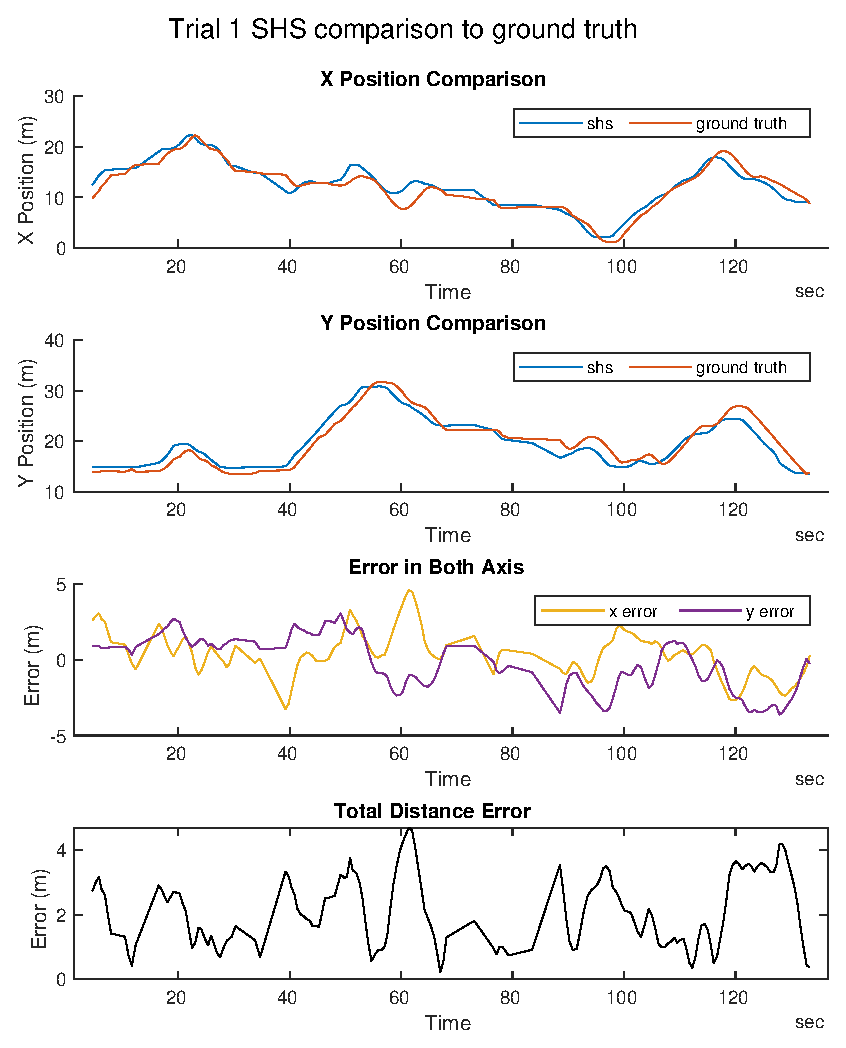
\includegraphics[width=\linewidth]{images/20201029_1040_trial1_shs_2}
		\caption{axis comparison}
		\label{fig:trial1_comparison}
	\end{subfigure}
	\caption{Qualitative SHS comparison of trial 1 with ground truth}
	\label{fig:trial1_shs_gt_comparison}
\end{figure}
\begin{figure}[]
	\centering
	\begin{subfigure}[t]{.45\textwidth}
		\centering
		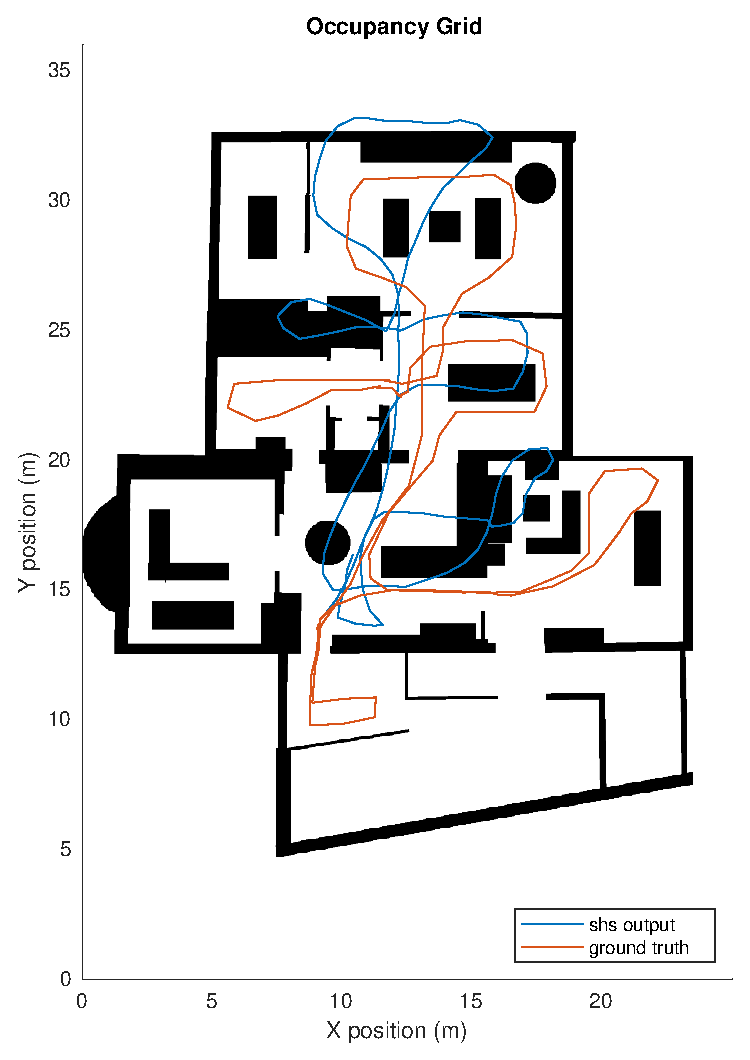
\includegraphics[width=0.9\linewidth]{images/20201029_1042_trial2_shs_1}
		\caption{trajectory comparison}
		\label{fig:trial2_on_map}
	\end{subfigure}
	\begin{subfigure}[t]{.45\textwidth}
		\centering
		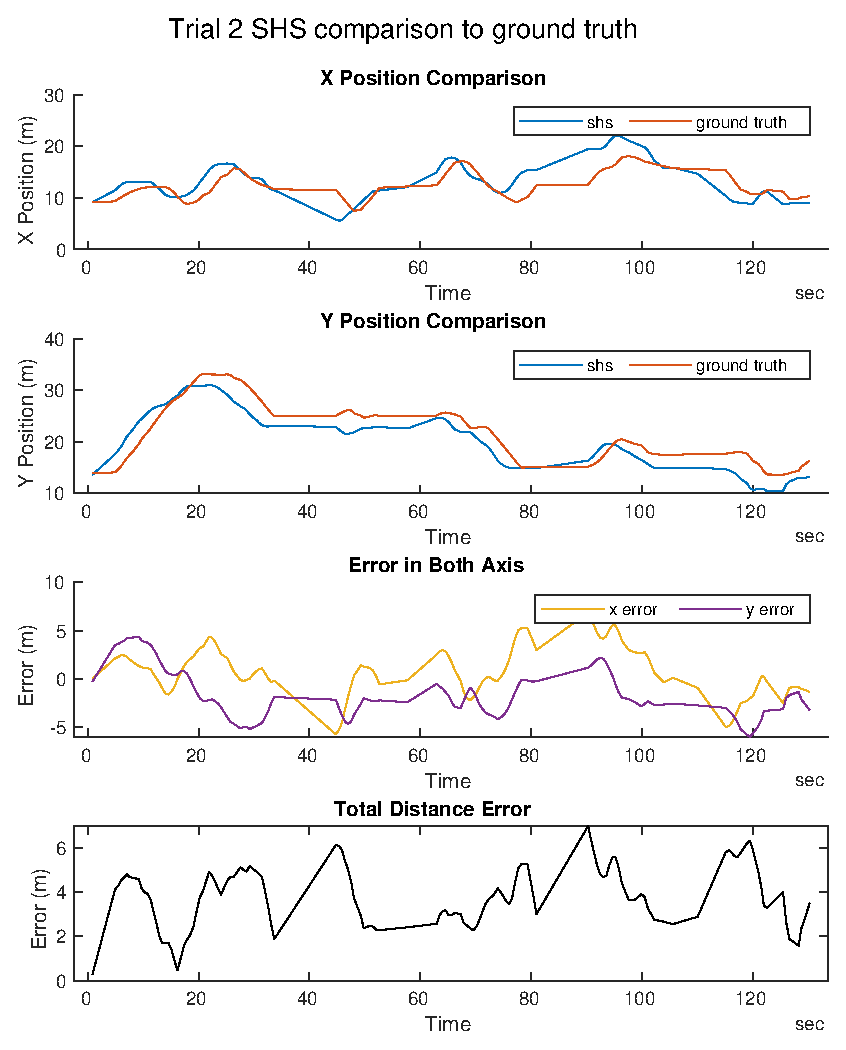
\includegraphics[width=\linewidth]{images/20201029_1042_trial2_shs_2}
		\caption{axis comparison}
		\label{fig:trial2_comparison}
	\end{subfigure}
	\caption{Qualitative SHS comparison of trial 2 with ground truth}
	\label{fig:trial2_shs_gt_comparison}
\end{figure}

\newpage
\subsection{Activity Recognition}
\textcolor{cyan}{
\begin{itemize}
	\item calculate the difference between the ground truth start of door interaction and the begin of the simple decision tree method outlined in the thesis
\end{itemize}}

\textcolor{red}{What do you think is also important to show about activity recognition}

\subsection{Particle Filter}
Using the output of the SHS, the method outlined in \cref{sec:method-pf} for the particle filter, and the map constructed for the indoor experiments, the indoor localization particle filter could be constructed. For initialization a known location on the map was available, around which the particles were distributed with a Bayesian profile. The output of the SHS was used to propagate the particles, with the map information removing particles that collided with the walls. \\
 

\subsubsection{Determining the estimate}
Within \cref{sec:method-pf} there are two approaches to determining the estimate. These are the maximum a posteriori (MAP) and the minimum mean square error (MMSE). While running the SHS particle filter method defined in this report, both forms of estimation proofed inadequate.
First, MMSE does not work well in situations in which there are multiple equal likely hypotheses. In such a case it will take the position in between the different hypothesis as the position estimate. A good example of this can be found in \cref{labellist}
\begin{figure}
	\centering
	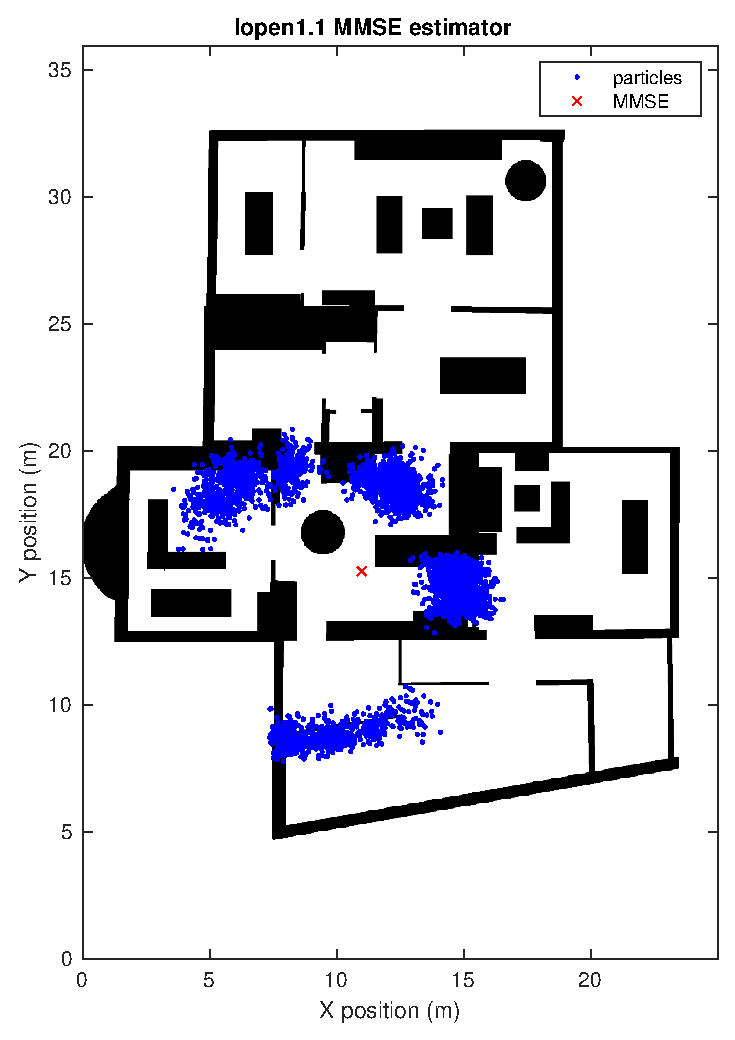
\includegraphics[width=0.5\linewidth]{images/20201108_1751_lopen1_1_MMSE_estimator}
	\caption{}
	\label{fig:lopen_11_mmse_estimator}
\end{figure}


Another approach was used in which the particles that survived the whole SHS trajectory made during the experiment were used. By recording the ancestors of these particles, the whole trajectory could be calculated by backtrack [\qn ?].

\textcolor{cyan}{
\begin{itemize}
	\item For this section I want to show MAP, RMSE and Ancestor Tracking (AT) on an example particle filter output to show why AT is better than th other two.
\end{itemize}}

\textcolor{red}{Do you think that I need a quantitative comparison between the different position estimate methods?}

\subsubsection{With activity}
During the experiment the possibility existed of recording at timestamp to indicate the beginning of interaction with a door within the indoor environment. This could be used as a ground truth comparison for eventual activity recognition, but also as a way of bypassing the activity recognition. At the different timestamps recorded, a particle filter measurement update can be initiated. Using this method the potential affect of activity recognition can be evaluated, by comparing the use of the timestamps with when they are not used. Two examples can be found in \cref{fig:shspf_trial2_shs_gt_comparison} and \cref{fig:shspf_trial3_shs_gt_comparison} which show the ground truth generated from video and the output of the particle filter using their respective SHS trajectories as input.

\textcolor{red}{the results here are only using the "ground truth" door detection method, but can be replaced by the actual activity recognition algorithm. I suspect that the results will not be very different since from AR testing, door activity is detected well using the method in \cref{sec:method-AR}}

\begin{figure}[H]
	\centering
	\begin{subfigure}[t]{.45\textwidth}
		\centering
		\begin{tikzpicture}
		\node[anchor=south west,inner sep=0] (image) at (0,0) {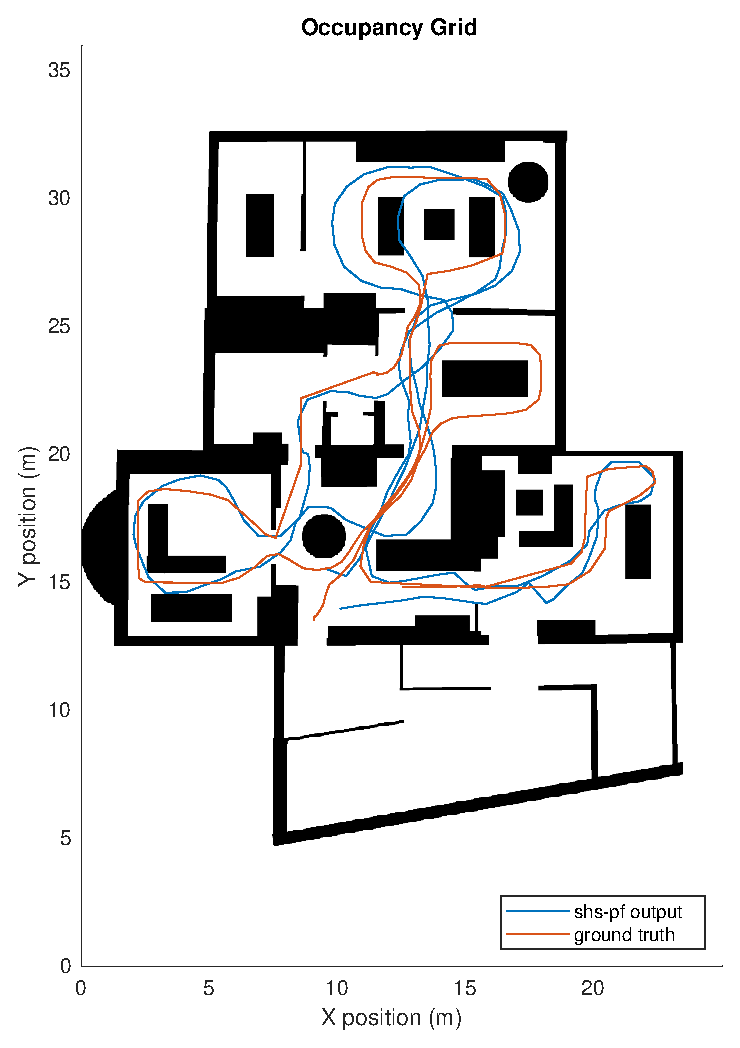
\includegraphics[width=0.9\textwidth]{images/20201029_1603_shs-pf_trial_1_2}};
		\begin{scope}[x={(image.south east)},y={(image.north west)}]
		\draw[green,ultra thick,rounded corners] (0.6,0.625) rectangle (0.73,0.66);
		\end{scope}
		\end{tikzpicture}		
		\caption{trajectory comparison}
		\label{fig:shspf_trial1_on_map}
	\end{subfigure}
	\begin{subfigure}[t]{.45\textwidth}
		\centering
		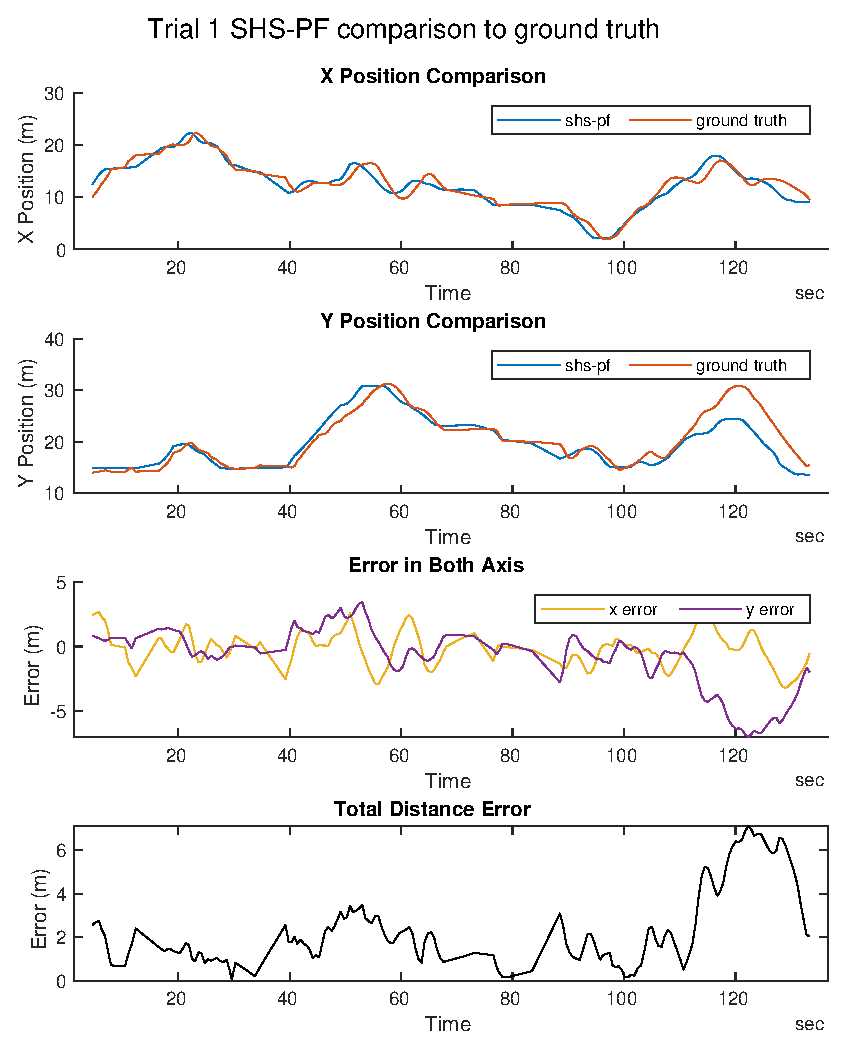
\includegraphics[width=\linewidth]{images/20201029_1603_shs-pf_trial_1_1}
		\caption{axis comparison}
		\label{fig:shspf_trial1_comparison}
	\end{subfigure}
	\caption{SHS-PF comparison of trial 1 with ground truth}
	\label{fig:shspf_trial1_shs_gt_comparison}
\end{figure}

\begin{figure}[H]
	\centering
	\begin{subfigure}[t]{.45\textwidth}
		\centering
		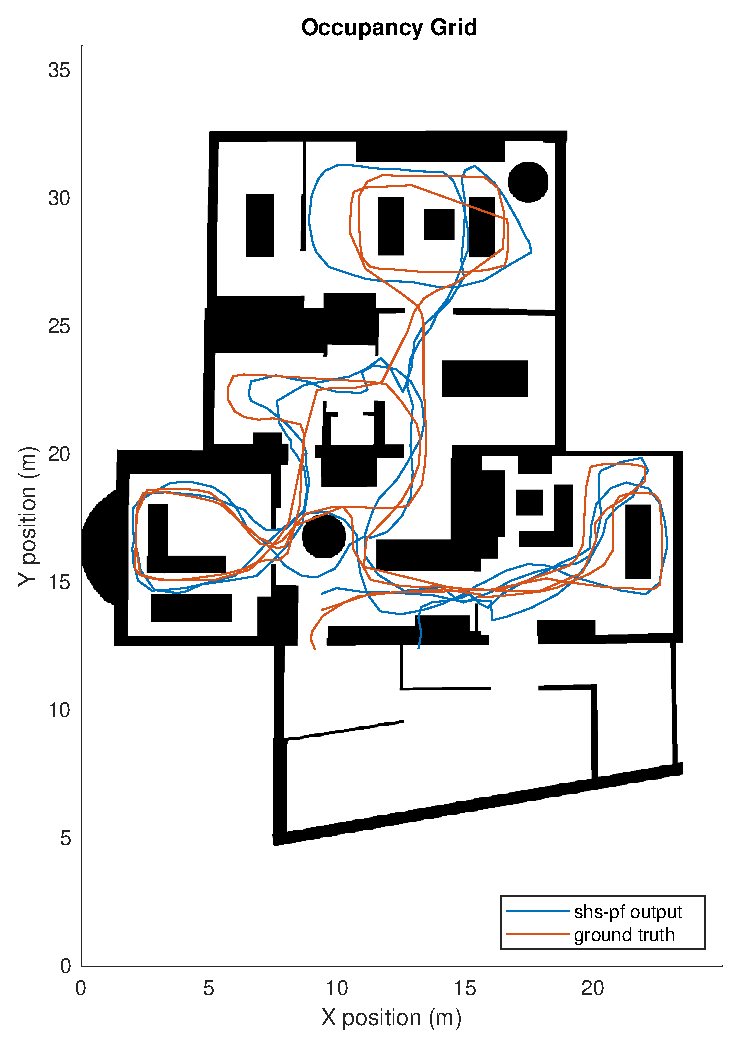
\includegraphics[width=0.9\linewidth]{images/20201029_1804_shs-pf_trial_3_2}
		\caption{trajectory comparison}
		\label{fig:shspf_trial3_on_map}
	\end{subfigure}
	\begin{subfigure}[t]{.45\textwidth}
		\centering
		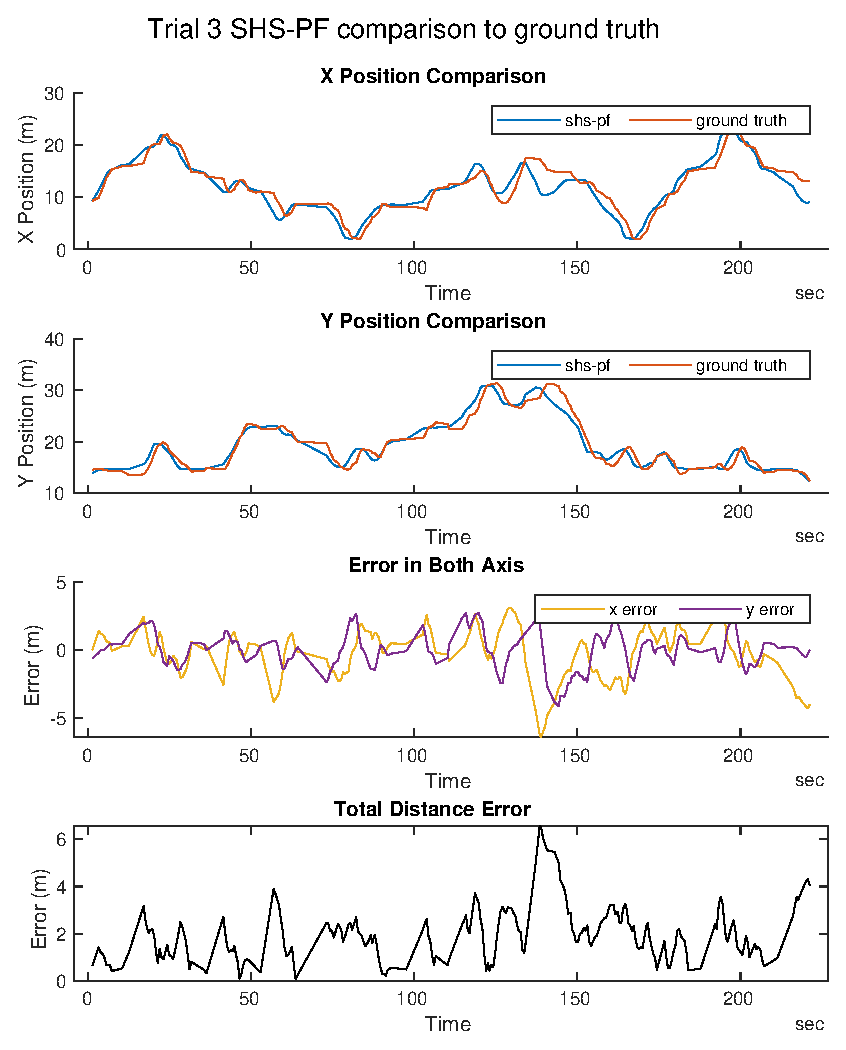
\includegraphics[width=\linewidth]{images/20201029_1804_shs-pf_trial_3_1}
		\caption{axis comparison}
		\label{fig:shspf_trial3_comparison}
	\end{subfigure}
	\caption{SHS-PF comparison of trial 3 with ground truth}
	\label{fig:shspf_trial3_shs_gt_comparison}
\end{figure}

\begin{figure}[H]
	\centering
	\begin{subfigure}[t]{.45\textwidth}
		\centering
		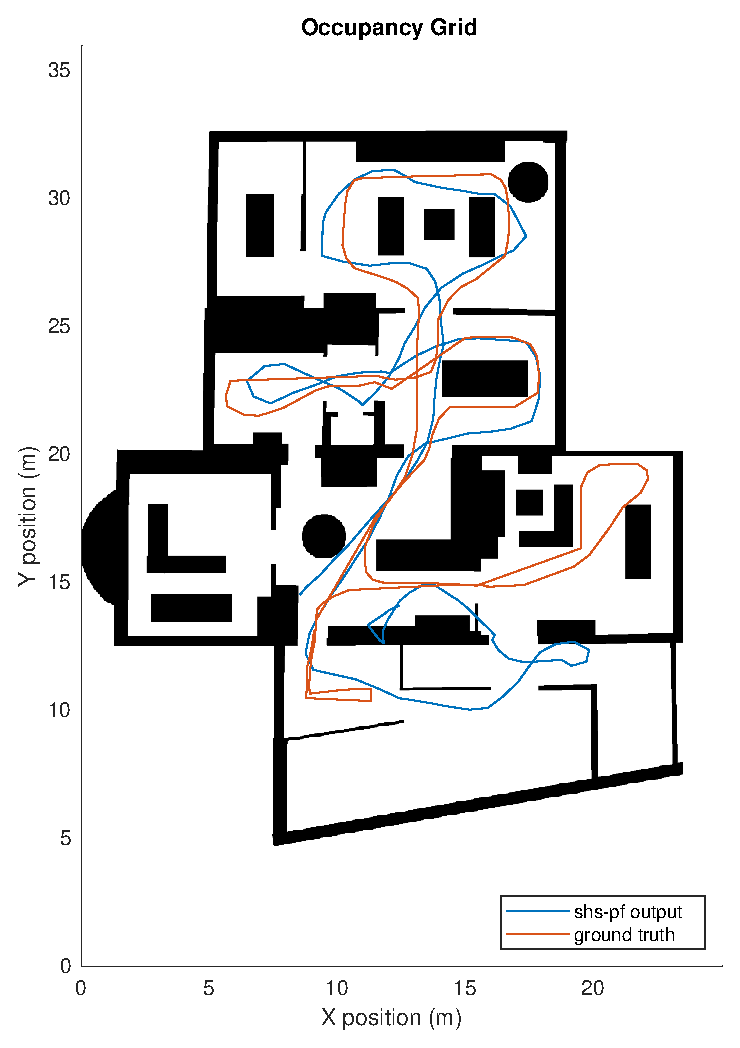
\includegraphics[width=0.9\linewidth]{images/20201107_1338_trial2_Occupancy_Grid}
		\caption{trajectory comparison}
		\label{fig:shspf_trial2_on_map}
	\end{subfigure}
	\begin{subfigure}[t]{.45\textwidth}
		\centering
		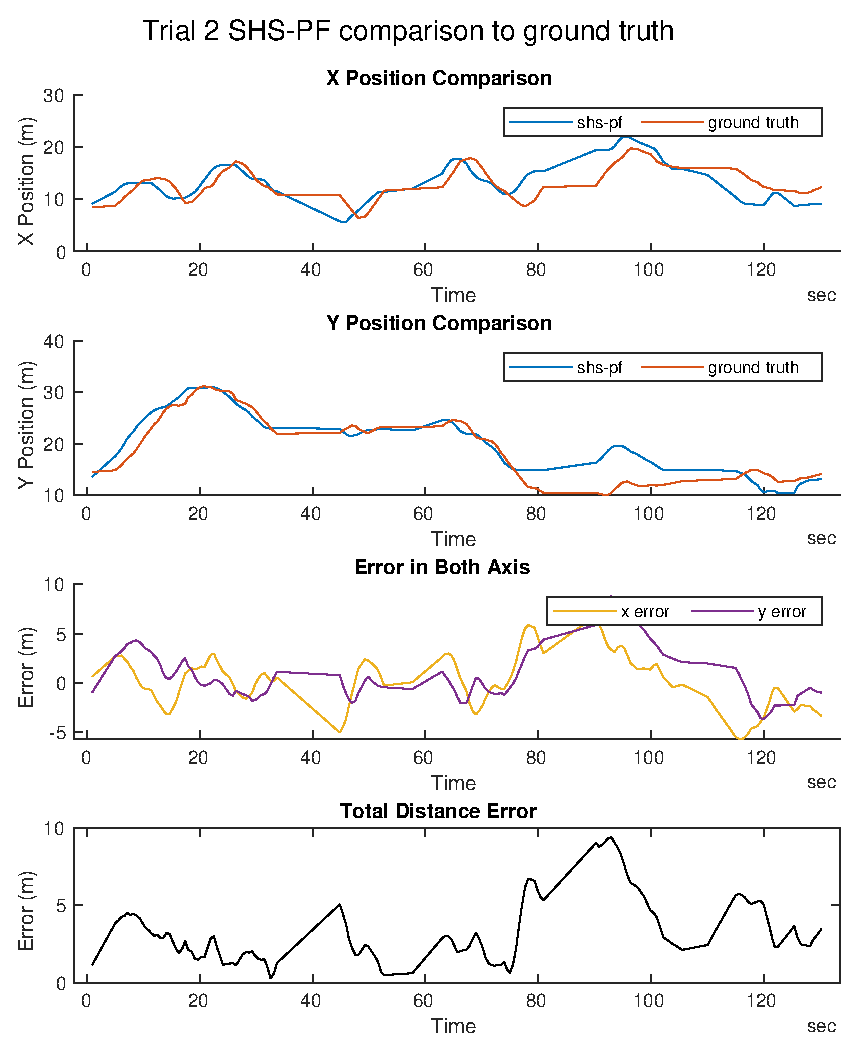
\includegraphics[width=\linewidth]{images/20201107_1338_trial2_Total_Distance_Error}
		\caption{axis comparison}
		\label{fig:shspf_trial2_comparison}
	\end{subfigure}
	\caption{SHS-PF comparison of trial 3 with ground truth}
	\label{fig:shspf_trial2_shs_gt_comparison}
\end{figure}

Running the particle filters with the same settings for lopen1.1-1.3, with 5 iterations each, generated the following results. The individual trajectories can be found in \cref{app:SHS-PF trials}.

\begin{figure}[H]
	\centering
	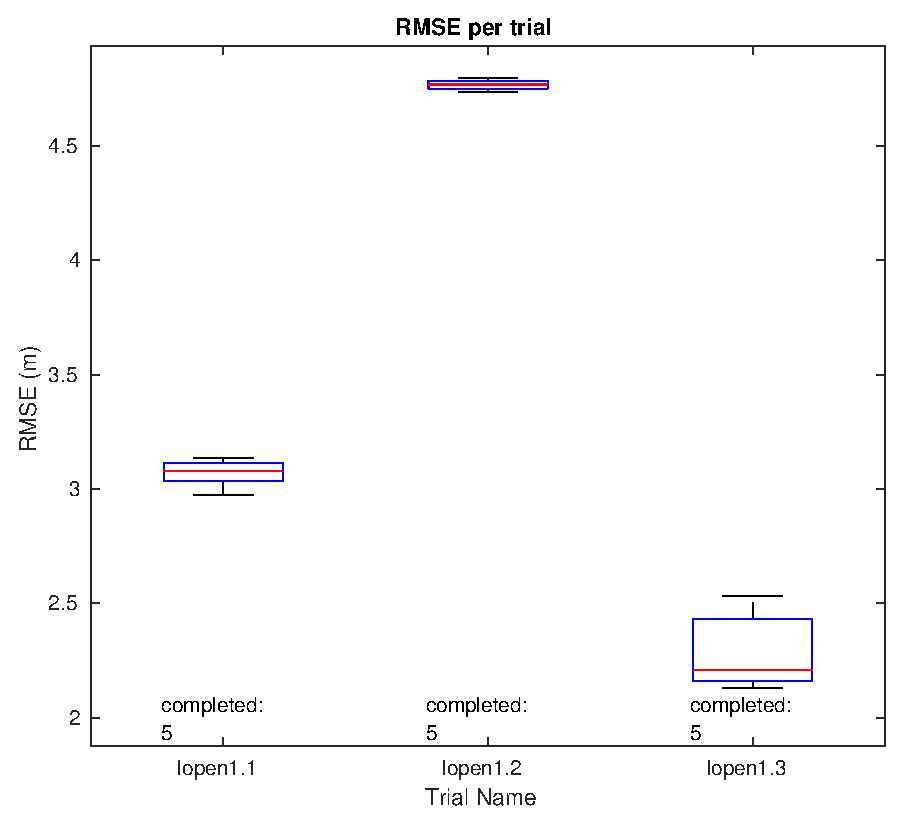
\includegraphics[width=0.6\textwidth]{images/20201103_1128_with_doors_2}
	\caption[Particle Filter position estimation performance with door interaction]{Particle Filter position estimation performance with door interaction measurment update, 5 itterations per trial. Number under "completed" indicates how many trials had particles surviving for the whole SHS trajectory. }
	
	\label{fig:pf_boxplot}
\end{figure}

\textcolor{purple}{
Things to notice:
\begin{itemize}
	\item All particle filters generate similar results and complete the whole trajectory
	\item the RMSE of lopen1.2 is quite high. The reason for this can be found in figure \cref{fig:shspf_trial2_shs_gt_comparison}, with the table that is circled in green. For all particle filter cases this object could not be circle, drastically adding to the RMSE of this trial.
	\item The particle did not perform consistently for lopen1.5 where it either worked well an example of which can be found in \cref{fig:shspf_trial3_shs_gt_comparison} , or diverged completely. I think this is due to the SHS trajectory input, with a focus on wrong step length estimation. This can be shown in a plot. What do you think?
\end{itemize}}

\textcolor{red}{there are about 4 more trials that can be processed, do you think that this is worthwhile?} \\
\textcolor{red}{I do not yet know how the particle filter will handle false positives. Can I discuss this with you during the meeting?}

\newpage
\subsubsection{Without activity}
The same SHS trajectory were used, however now door interaction landmarks were not used as measurement update. The results can be found in \cref{fig:pf_boxplot_no_doors}.

\begin{figure}[H]
	\centering
	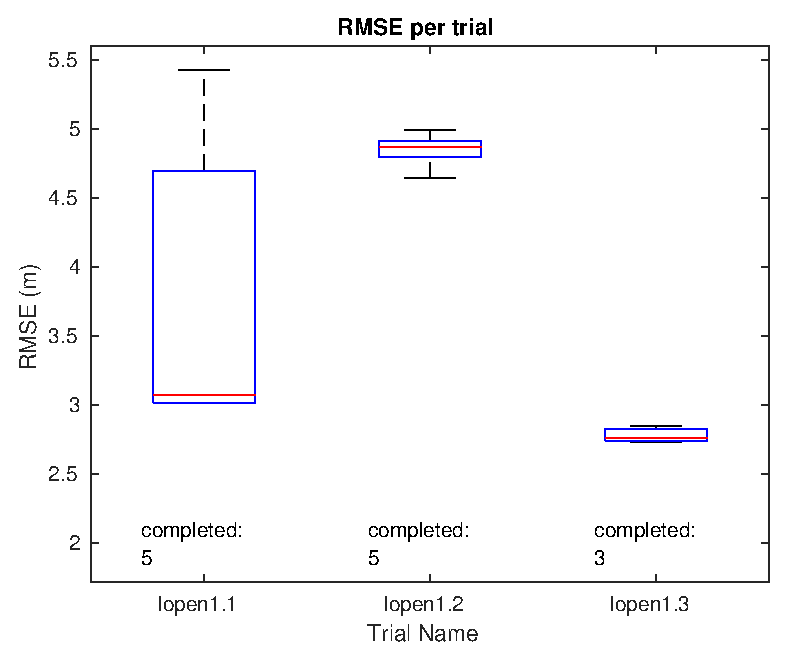
\includegraphics[width=0.7\textwidth]{images/20201103_1128_with_doors_1}
	\caption[Particle Filter position estimation performance without door interaction]{Particle Filter position estimation performance without door interaction measurment update, 5 itterations per trial. Number under "completed" indicates how many trials had particles surviving for the whole SHS trajectory.}
	\label{fig:pf_boxplot_no_doors}
\end{figure}

\textcolor{purple}{
things to notice
\begin{itemize}
	\item Trial one has very different RMSE value per run
	\item Strangely it did not have much effect on lopen1.2
	\item Although the RMSE of lopen1.3 is similar to the one with door activity two of the 5 trials did not complete the SHS track. This means that all particles.
	\item So far this does indicate that having activity recognition does help with position estimation within a particle filter
\end{itemize}}
